\chapter{呼吸代谢和能量转换}

\section{呼吸作用的基本概念}
\begin{enumerate}
    \item 呼吸作用的生理意义:
    \begin{enumerate}
        \item 为植物生命活动提供能量;
        \item 为植物体内其他重要有机物质合成提供原料,是植物代谢的中心;
        \item 在植物抗病免疫方面起重要作用。
    \end{enumerate}
    \item 呼吸代谢的过程:\uline{底物的降解(底物氧化)}、\uline{能量产生(末端氧化)}。
    \item \textbf{呼吸商(RQ)}:呼吸底物在呼吸过程中所释放的CO$_2$的量和吸收的O$_2$的量之间的比值。糖类RQ$=1$,油脂、蛋白质RQ$<1$。
    \[
        \text{RQ}=\frac{\text{释放的CO}_2\text{的量}}{\text{吸收的O}_2\text{的量}}
    \]
    \item \textbf{呼吸强度/呼吸速率}:单位质量的呼吸材料在单倍时间内进行呼吸所消耗的O$_2$或释放的CO$_2$的量。
\end{enumerate}

\section{植物呼吸代谢途径}
\subsection{淀粉和蔗糖的降解}
\begin{enumerate}
    \item 淀粉降解的途径:\uline{淀粉磷酸化分解}、\uline{淀粉水解}。
    \item 淀粉降解的场所:\uline{质体(叶绿体、淀粉体)}、\uline{细胞质}。淀粉在质体中以\uline{囊泡包裹}形式运出。
    \item 淀粉降解相关酶:
    \begin{enumerate}
        \item \textbf{α-淀粉酶}:攻击完整淀粉粒,随机作用于直链部分α-1,4-糖苷键;
        \item \textbf{β-淀粉酶}:作用于淀粉非还原端α-1,4-糖苷键;
        \item \textbf{淀粉磷酸解酶}:作用于淀粉非还原端α-1,4-糖苷键;
        \item \textbf{脱支酶(支链淀粉酶)}:作用于支链部分α-1,6-糖苷键。
    \end{enumerate}
    \item 蔗糖降解的场所:\uline{细胞质}。
    \item 蔗糖降解相关酶:
    \begin{enumerate}
        \item \textbf{蔗糖合酶}:催化形成UDP-G、果糖;
        \item \textbf{蔗糖转化酶}:催化形成葡萄糖。
    \end{enumerate}
\end{enumerate}
\subsection{糖酵解途径}
\begin{enumerate}
    \item \textbf{糖酵解(EMP)途径}总反应式:
    \[\begin{aligned}
        \text{葡萄糖}+2\text{NAD}^+&+2\text{ADP}^{2-}+2\text{H}_2\text{PO}^{4-}\\&\to 2\text{丙酮酸}+2\text{NADH}+2\text{H}^++2\text{ATP}^{3-}+2\text{H}_2\text{O}
    \end{aligned}\]
    \item 无氧呼吸后续过程:
    \begin{enumerate}
        \item 酒精发酵:丙酮酸氧化脱羧为乙醛,\textbf{乙醇脱氢酶}利用\uline{NADH}进一步把乙醛还原为乙醇。此过程发生在大多数植物和一些产乙醇的微生物中(如酵母)。动物中没有该过程。
        \item 乳酸发酵:丙酮酸在\textbf{乳酸脱氢酶}作用下,利用\uline{NADH}将丙酮酸还原为乳酸。此过程发生在少数植物(如马铃薯块茎)、动物骨骼肌及部分微生物中(主要是细菌)。
    \end{enumerate}
    \item 糖酵解过程:***
\end{enumerate}
\subsection{三羧酸循环}
\begin{enumerate}
    \item \textbf{丙酮酸转运器}位于线粒体内膜,介导丙酮酸进入线粒体基质(线粒体外膜通透性高,丙酮酸可以直接穿越)。
    \item \textbf{三羧酸循环}总反应式:
    \[\begin{aligned}
        \text{CH}_3\text{CO}\sim\text{SCoA}+3\text{NAD}^+&+\text{FAD}+\text{GDP}+\text{Pi}+2\text{H}_2\text{O}\\\to 2\text{CO}_2+3\text{NADH}&+3\text{H}^++\text{FADH}_2+\text{HS}\sim\text{CoA}+\text{ATP/GTP}
    \end{aligned}\]
    \item 植物三羧酸循环的特点:
    \begin{enumerate}
        \item 由琥珀酰辅酶A合成酶催化的从琥珀酰辅酶A(Succinyl-CoA)转化为琥珀酸(Succinic acid)的反应,\uline{在植物中是生成ATP},而在动物中生成的是GTP。
        \item \textcolor{red}{NAD$^+$苹果酸酶:}在植物线粒体中普遍存在,它催化\uline{苹果酸的氧化脱羧反应}($\text{苹果酸}+\text{NAD}^+\to\text{丙酮酸}+\text{CO}_2+\text{NADH}$),这在其他生物中不存在。NAD+苹果酸酶的存在使植物可以在缺少丙酮酸的情况下,\uline{完全氧化有机酸},例如苹果酸、柠檬酸等。
    \end{enumerate}
\end{enumerate}
\subsection{乙醛酸循环}
\begin{enumerate}
    \item \textbf{乙醛酸循环}:使脂肪酸氧化释放的乙酰CoA转变成琥珀酸和苹果酸,再经草酰乙酸步骤转变成糖或补充三羧酸循环的琥珀酸和苹果酸。
    \item \textcolor{red}{乙醛酸循环的过程:}
    \begin{center}
        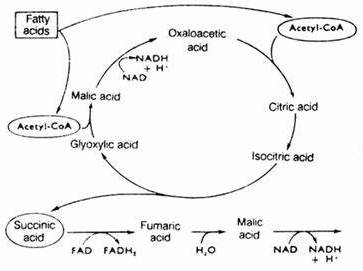
\includegraphics[width=.5\textwidth]{figure/乙醛酸循环.jpeg}
    \end{center}
    \item 乙醛酸循环总反应式:
    \[
        2\text{乙酰CoA}+\text{NAD}^+\to\text{琥珀酸}+2\text{CoA}+\text{NADH}+\text{H}^+
    \]
    \item 植物乙醛酸循环在\uline{乙醛酸循环体}(一种\uline{微体},与过氧化物酶体同源)和\uline{线粒体}中协同进行,可以说是三羧酸循环的辅佐途径。
    \item 动物细胞中没有乙醛酸体,无法将脂肪酸转变为糖。 
    \item 乙醛酸循环在异柠檬酸与琥珀酸、苹果酸间搭了一条捷径。
    \item \textcolor{red}{乙醛酸循环的化学历程:}
    \begin{enumerate}
        \item 脂肪酸在乙醛酸体内经过β-氧化分解为乙酰CoA,后者与\uline{草酰乙酸}缩合为\uline{柠檬酸},进一步形成\uline{异柠檬酸};
        \item 异柠檬酸在异柠檬酸裂解酶的作用下分解为\uline{琥珀酸}和\uline{乙醛酸};
        \item \uline{乙醛酸}与\uline{乙酰CoA}在苹果酸合成酶催化下生成\uline{苹果酸},脱氢形成\uline{草酰乙酸},构成循环;
        \item 琥珀酸由乙醛酸体转移到线粒体参与三羧酸循环,或转移到细胞质生成\uline{磷酸烯醇式丙酮酸(PEP)}参与\uline{糖异生}。(但也有人认为是苹果酸进入的细胞质。)
    \end{enumerate}
    \item \textcolor{red}{乙醛酸循环的作用:}
    \begin{enumerate}
        \item 通过乙醛酸途径使乙酰-CoA转变为草酰乙酸从而进入柠檬酸循环。
        \item 使萌发的种子将贮存的甘油三脂,通过乙酰-CoA转变为葡萄糖。 
    \end{enumerate}
    \item \uline{蓖麻种子}萌发时,乙醛酸循环产物的外运形式是苹果酸,苹果酸或进入细胞质参与糖异生,或通过“\textbf{苹果酸穿梭}”进入线粒体。
    \item 与糖异生的关系:
    \[
        \text{油脂}\overset{\text{β-氧化}}\longrightarrow\text{乙酰CoA}\overset{\text{乙醛酸循环}}\longrightarrow\text{草酰乙酸}\overset{糖异生}\longrightarrow\text{糖}
    \]
\end{enumerate}

\subsection{磷酸戊糖途径}
\begin{enumerate}
    \item \textbf{磷酸戊糖(PPP)途径}:以\uline{6-磷酸葡萄糖}开始,在\textbf{6-磷酸葡萄糖脱氢酶}(限速酶)催化下形成\uline{6-磷酸葡萄糖酸},进而代谢生成\uline{磷酸戊糖}为中间代谢物的过程。
    \item 磷酸戊糖途径总反应式:
    \[
        \text{G-6-P}+12\text{NADP}^++7\text{H}_2\text{O}\to 6\text{CO}_2+12\text{NADPH}+12\text{H}^++\text{H}_3\text{PO}_4
    \]
    \item 磷酸戊糖途径的意义:
    \begin{enumerate}
        \item \uline{产生NADPH},为各种合成反应提供还原力,比如参与脂肪酸和固醇类物质的合成;
        \item 为许多物质的合成提供原料:重要的\uline{5-P-核糖是核苷酸合成的原料};另外比如,\uline{4-P-赤藓糖是氨基酸合成的原料};
        \item 一系列中间产物及酶类与光合作用中卡尔文循环的大多数中间产物和酶相同,因而磷酸戊糖途径可与光合作用联系起来,并实现\uline{某些单糖间的互变}。
        \item 该途径是由葡萄糖直接氧化起始的可单独进行氧化分解的途径,也是\uline{戊糖代谢的主要途径},因此可以和EMP-TCA相互补充、相互配合。
    \end{enumerate}
\end{enumerate}

\section{电子传递链}
\begin{enumerate}
    \item 电子传递链的组成:
    \begin{enumerate}
        \item 复合体I:NADH-泛醌Q还原酶;
        \item 复合体II:琥珀酸-泛醌Q还原酶;
        \item 复合体III:细胞色素还原酶;
        \item 复合体IV:细胞色素氧化酶。
    \end{enumerate}
    \item 电子传递顺序:
    \begin{enumerate}
        \item NAD(P)H氧化呼吸链:NADH$\to$复合体I$\to$Q$\to$复合体III$\to$细胞色素C$\to$复合体IV$\to$O$_2$;
        \item FADH$_2$氧化呼吸链:FADH$_2\to$复合体II¥$\to$Q$\to$复合体III$\to$细胞色素C$\to$复合体IV$\to$O$_2$。
    \end{enumerate}
    \item 电子传递抑制剂:
    \begin{center}
        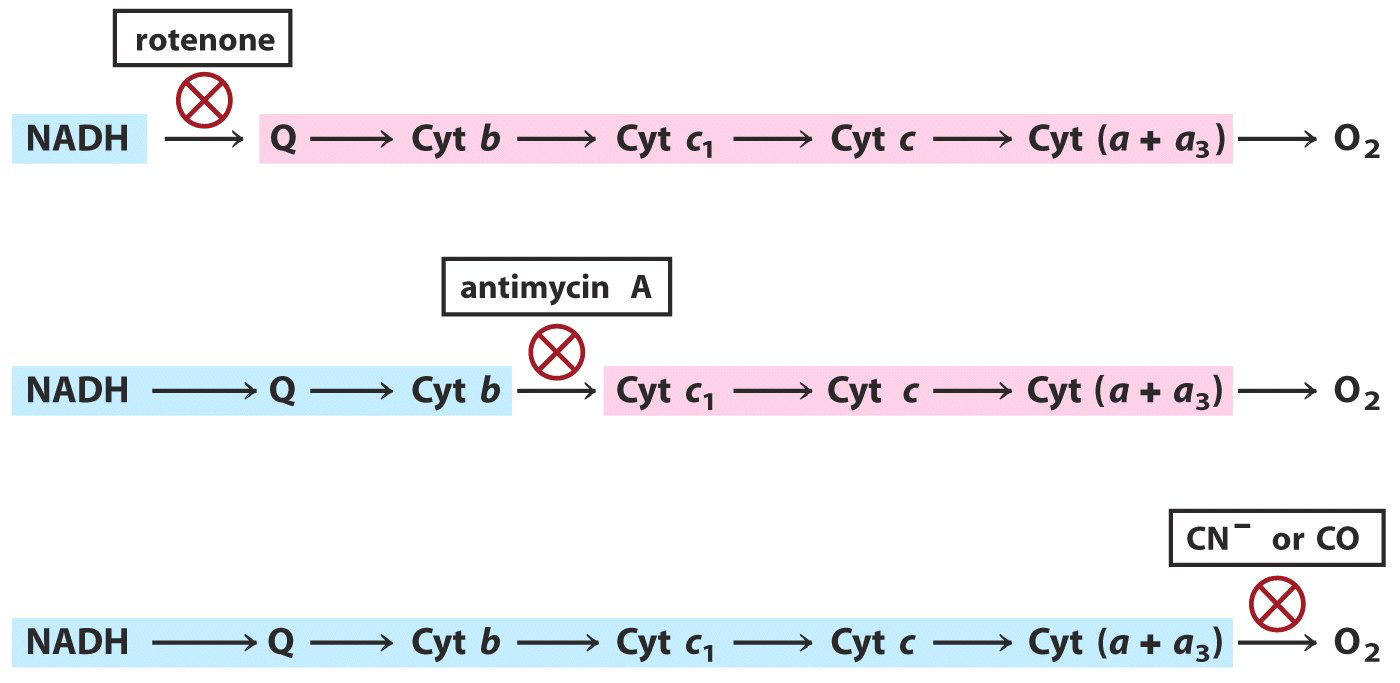
\includegraphics[width=.8\textwidth]{figure/电子传递抑制剂.png}
    \end{center}
\end{enumerate}

\section{氧化磷酸化}
\begin{enumerate}
    \item 底物水平磷酸化:
    \begin{enumerate}
        \item 1,3-二磷酸甘油酸$\overset{\text{3-磷酸甘油酸激酶}}\longrightarrow$3-磷酸甘油酸+ATP;
        \item 磷酸烯醇式丙酮酸$\overset{\text{丙酮酸激酶}}\longrightarrow$丙酮酸+ATP;
        \item 琥珀酰-CoA + H$_3$PO$_4$ + GDP/ADP$\overset{\text{琥珀酰-CoA合成酶}}\longrightarrow$琥珀酸 + CoA + GTP/ATP。
    \end{enumerate}
    \item 电子传递体系磷酸化:末端氧化,有\textbf{能量偶联假说},其下有三个学说:\uline{化学耦联学说}、\uline{结构耦联学说}、\uline{化学渗透学说}。
    \begin{enumerate}
        \item 化学偶联假说:认为电子传递过程产生一种活泼的高能共价中间物。它随后的裂解驱动氧化磷酸化作用。
        \item 构象偶联假说:认为电子传递使线粒体内膜蛋白质组分发生了构象变化,形成一种高能形式。这种高能形式通过ATP的合成而恢复其原来的构象。
        \item 化学渗透学说:认为电子传递释放出的自由能和ATP合成是与一种跨线粒体的质子梯度相偶联的。
    \end{enumerate}
    \item 线粒体外NADH的穿梭:
    \begin{itemize}
        \item 胞液中的3-磷酸甘油醛/磷酸二羟丙酮或乳酸/乙醇脱氢(糖酵解),均可产生NADH。
        \item 这些NADH可经-磷酸甘油穿梭和苹果酸天冬氨酸穿梭两种方式进入线粒体氧化磷酸化过程。
    \end{itemize}
\end{enumerate}

\section{其他末端氧化酶系}
\begin{enumerate}
    \item 抗氰氧化酶系统(线粒体内):有些植物细胞线粒体内存在抗氰氧化酶,当氰化物作用于复合体IV,阻断正常呼吸链时,电子可以从复合体III的Cytb直接传给抗氰氧化酶(绕开细胞色素c和复合体IV细胞色素氧化酶)再交给氧。其生理意义有:
    \begin{enumerate}
        \item 有利于低温地区传粉和种子萌发(放热);
        \item 抵御逆境;
        \item 分流电子:当呼吸底物积累大于生长、储存、ATP合成需要时,通过该途径将多余能量消耗掉。
    \end{enumerate}
    \item 多酚氧化酶系统(线粒体外):此酶与植物组织受伤反应有关,植物组织受伤后多酚氧化酶活力增高,呼吸作用增强;植物受病菌侵害时,多酚氧化酶活力也增高,有利于把酚类化合物氧化为醌,醌对病菌有毒害而起抗病作用。
    \item 抗坏血酸氧化酶系统(线粒体外):可能与植物的抗病有关。
    \[
        \text{抗坏血酸}+\text{O}_2\overset{\text{抗坏血酸氧化酶}}\longrightarrow\text{脱氢抗坏血酸}+\text{H}_2\text{O}
    \]
    \item 超氧化物歧化酶(SOD):清除自由基活性氧,在植物胞质和叶绿体、动物的红细胞和其它细胞、细菌中都存在。
    \item 乙醇酸氧化酶:一种黄素蛋白,存在于过氧化体中,催化乙醇酸氧化为乙醛酸的反应,在光呼吸中起重要作用。此过程中会产生过氧化氢,在过氧化氢酶催化下产生具有强氧化能力的新生态氧,并释放于根的周围,形成一层氧化圈。
\end{enumerate}